% Formato de la hoja
\documentclass[letterpaper, 12pt, oneside]{book} % carta, letra: 12
\renewcommand{\baselinestretch}{1.5} % Interlineado general
\usepackage[margin=2.5cm, top=4cm, left=4cm]{geometry}

% Fuente 
%\usepackage{fontspec}
%\setmainfont{Arial}
\usepackage{helvet}
\renewcommand{\familydefault}{\sfdefault}
\usepackage[T1]{fontenc}

% Para insertar Imágenes
\usepackage{graphicx}
\graphicspath{{./figuras/}}

% Paquetes
\usepackage[english, spanish, es-tabla]{babel} % configuración en español
\usepackage{wrapfig} % envolver imágenes alrededor de texto
\usepackage{setspace} % opciones de espaciado
\usepackage{parskip} % formato de texto con salto de párrafo
\usepackage{tabularx} % mejores tablas
\usepackage[dvipsnames, table]{xcolor} % definir colores
\usepackage{hyperref} % insertar enlaces dentro del documento
\usepackage{xurl} % insertar url's directamente
\usepackage{verbatim} % para usar texto monoespaciado como código
\usepackage{listings} % para formatear texto como código
\usepackage{enumitem} % para configurar los entornos enumerate, itemize.
\usepackage[titletoc]{appendix} % definir el apéndice
\usepackage[labelfont=bf,justification=raggedright,singlelinecheck=false]{caption}
\usepackage{fancyhdr}
\usepackage{lastpage}
\usepackage{titlesec}
\usepackage[titles]{tocloft}
\usepackage{etoc}


% Para la bibliografía
\usepackage[backend=biber, style=apa, sorting=nyt]{biblatex}
\usepackage{csquotes}
\addbibresource{referencias.bib}

\definecolor{light-gray}{gray}{0.95}

\titlespacing*{\chapter}{0pt}{0pt}{20pt}  % centrado, sin espacio arriba
% \titlespacing*{name=\chapter,numberless}{0pt}{0pt}{20pt}  % centrado, sin espacio arriba

\titleformat{\chapter}[display] % Estilo de los capítulos
  {\bfseries\Large\centering}
  {\MakeUppercase\chaptername\ \thechapter}
  {10pt}
  {\titlerule\MakeUppercase}

\titleformat{name=\chapter,numberless}[block]
  {\bfseries\Large\centering}        % mismo estilo
  {}                                % sin número
  {0pt}                             % separación antes de la línea
  {\MakeUppercase}                  % título en mayúsculas
  [\vspace{10pt}\titlerule]         % línea después del título
\titlespacing*{name=\chapter,numberless}{0pt}{0pt}{20pt}

\titleformat{\section}[block]
  {\Large\bfseries}
  {\thesection}
  {10pt}
  {\MakeUppercase}

\titleformat{\subsection}[block]
  {\large\bfseries}
  {\thesubsection}
  {10pt}
  {\MakeUppercase}

\titleformat{\subsubsection}[block]
  {\normalsize\bfseries}
  {\thesubsubsection}
  {10pt}
  {\MakeUppercase}

\etocsettocstyle{\chapter*{Índice General}}{}

% 'Capítulo X: ' en Índice
\renewcommand{\cftchappresnum}{Capítulo~}
\renewcommand{\cftchapaftersnum}{:\ }
\renewcommand{\cftchapnumwidth}{6em}

% Colores de Enlaces (Links)
\hypersetup{
    colorlinks,
    citecolor=black,
    filecolor=black,
    linkcolor=black,
    urlcolor=blue
}

% Configuración del estilo de código
\lstset{
    basicstyle=\ttfamily\footnotesize,
    keywordstyle=\color{blue}\bfseries,
    commentstyle=\color{gray}\itshape,
    stringstyle=\color{teal},
    backgroundcolor=\color{light-gray},
    numbers=left,
    numberstyle=\scriptsize,
    stepnumber=1,
    numbersep=8pt,
    breaklines=true,
    tabsize=4,
    showstringspaces=false
    aboveskip=5pt,
    belowskip=5pt,
    lineskip=-1pt
}

% Modificar Headers y Footers
\pagestyle{fancy}
\fancyhf{}
\renewcommand{\headrulewidth}{0pt} % quitar línea superior
\fancyfoot[R]{\thepage}
\fancypagestyle{plain}{}

%%% COMANDOS PERSONALIZADOS %%% 

% \sourcefig{nombre}{año}{url} : para insertar una fuente a una figura
\newcommand{\sourcefig}[3]{%
  \caption*{%
    \small\textcolor{gray}{%
      Fuente: #1%
      \if\relax\detokenize{#2}\relax\else, #2\fi%
      \if\relax\detokenize{#3}\relax%
        % No hay URL → no mostrar "Enlace:"
      \else%
        , Enlace: \url{#3}%
      \fi%
    }%
  }%
}
% \code{} : para insertar una palabra de texto monoespaciada, como documentación
\newcommand{\code}[1]{\colorbox{light-gray}{\texttt{#1}}}


%%%%%%%%%%%%%%%%%%%%%%%%%%%%%%%%%%%%%%%%%%%%%%%%%%%%%%%%%%%%%%%%%%%%
% INICIO DOCUMENTO %%%%%%%%%%%%%%%%%%%%%%%%%%%%%%%%%%%%%%%%%%%%%%%%%
%%%%%%%%%%%%%%%%%%%%%%%%%%%%%%%%%%%%%%%%%%%%%%%%%%%%%%%%%%%%%%%%%%%%

\begin{document}

    % ================ Preliminares ====================
    \frontmatter % números romanos

    \begin{titlepage}
    \begin{wrapfigure}[5]{L}{2cm}
        
\includegraphics[width=2cm]{figuras/logo_utem.png}
    \end{wrapfigure}

    {\setstretch{1.1}
        \noindent UNIVERSIDAD TECNOLÓGICA METROPOLITANA\\
        FACULTAD DE INGENIERÍA\\
        DEPARTAMENTO DE INFORMÁTICA\\
        ESCUELA DE INFORMÁTICA\\
        CARRERA INGENIERÍA EN INFORMÁTICA
        \vfill
    }

    % TÍTULO
    \begin{center}
        \setstretch{2} % título a doble espacio si utiliza más de un reglón
        \textbf{\Large REINGENIERÍA DE UN SISTEMA DE GESTIÓN DE UNIFORMES CORPORATIVOS} 
    \end{center}

    \vfill
    
    \begin{center}
        \textbf{\large TRABAJO DE TITULACIÓN PARA OPTAR AL TÍTULO DE INGENIERO EN INFORMÁTICA} 
    \end{center}
        
    \vfill

    \begin{flushright}
        \textbf{\large AUTORES:} 

        ARANEDA MELLA, GERARDO GABRIEL \\
        GÓMEZ RODRÍGUEZ, ANDRÉS \\
        JIMÉNEZ ROMERO, NICOLÁS 
        
        \textbf{\large PROFESOR GUÍA:}
        
        YELKA RUIZ ROCHA
        
    \end{flushright}
    
    \vspace{0.5in}

    \begin{center}
        \small SANTIAGO - CHILE \\
        2025
    \end{center}

\end{titlepage}

    \setcounter{page}{2}

    \begin{singlespace}
    \begin{center}
        \large \textbf{Autorización para la Reproducción del Trabajo de Titulación}
    \end{center}
    \vspace{1cm}
    
    1. Identificación del trabajo de titulación
    
    Nombre del(os) alumno(s)
    
    \dotfill \\
    Rut \dotfill \\
    Dirección \dotfill \\
    E-mail \dotfill \\
    Teléfono \dotfill

    Título de la tesis

    \dotfill \\
    Escuela \dotfill \\
    Carrera o programa \dotfill \\
    Título al que opta \dotfill

    2. Autorización de Reproducción %seleccionar una opción

    % Este trabajo de titulación no puede reproducirse o transmitirse bajo ninguna forma o por ningún medio o procedimiento, sin permiso escrito del(os) autor(es), exceptuando la cita bibliográfica, resumen y metadatos que acreditan al trabajo y a su(s) autor(es).

    Se autoriza la reproducción total o parcial de este trabajo de titulación, con fines académicos, por cualquier medio o procedimiento, incluyendo la cita bibliográfica que acredita al trabajo y a su autor.
    
    En consideración a lo anterior, se autoriza su reproducción de forma (marque con una X):

    \begin{table}[h]
        \centering
        \setstretch{1}
        \renewcommand{\arraystretch}{2}
        \newcolumntype{Y}{>{\centering\arraybackslash}X}

        \begin{tabularx}{\textwidth}{|p{2cm}|X|}
            \hline
             & Inmediata \\
            \hline
             & A partir de la siguiente fecha: \rule{2cm}{0.4pt} (mes/año) \\
            \hline
        \end{tabularx}
    \end{table}

    \vfill

    Fecha: \rule{4cm}{0.4pt} \hfill Firma: \rule{4cm}{0.4pt} \hspace{2cm}

    \vspace{1cm}

    Esta autorización se otorga en el marco de la ley N°17.336 sobre Propiedad Intelectual, con carácter gratuito y no exclusivo para la Institución.
    
\end{singlespace}

    \hfill
\begin{minipage}{0.5\textwidth}
    \setstretch{1}
    \Large
        
    NOTA OBTENIDA: 

    \vspace{3cm}
    
    \rule{6.6cm}{0.4pt} \\
    Firma y timbre autoridad \\ responsable
\end{minipage}
\vfill


    % \chapter*{Dedicatoria}

    \begin{singlespace}
        \tableofcontents \newpage
        \listoftables \newpage
        \listoffigures \newpage
    \end{singlespace}

    % \textbf{RESUMEN:}

El resumen debe dar cuenta en forma clara y simple el contenido de la obra, permite determinar la pertinencia del trabajo y decidir al lector si el documento es de su interés. Se constituye de una descripción simple, breve y concisa de:

\begin{enumerate}
    \item El objetivo del trabajo
    \item Método o procedimiento utilizado
    \item Conclusiones o resultados obtenidos
\end{enumerate}

El resumen debe ser informativo y expresar en el mínimo número de palabras la mayor cantidad de información posible sobre el contenido del trabajo de titulación y su extensión máxima es de una página.

También incluye las palabras claves, que son términos temáticos que más destacan del trabajo, los cuales permiten su búsqueda e identificación en distintos recursos de información, como catálogos de biblioteca, motores de búsqueda y bases de datos.

\textbf{PALABRAS CLAVE:}

Repositorio, Universidad Tecnológica Metropolitana, software libre, preservación digital, acceso abierto.

\newpage

\textbf{ABSTRACT:}

LO MISMO QUE EL RESUMEN, PERO EN INGLÉS

In Chile, as in many other countries, the number of institutional repositories has grown steadily according to the need of information units and institutions in general to group, manage and preserve their institutional and scientific production, that is why this work addresses the elaboration of a best practices manual and general guidelines for the implementation of an institutional repository at Universidad Tecnológica Metropolitana, with emphasis in its value as a tool for supporting teaching and learning. It takes into account the situation of Chilean universities repositories and justify the need for implementing one at UTEM’s library system. Finally, it gives general guidelines for its implementation, which includes software, hardware, procedures and legal regulations.

\textbf{KEYWORDS:}

Repository, Universidad Tecnológica Metropolitana, open source software, digital preservation, open access.

    % ================ Cuerpo ==========================
    \mainmatter % números arábigos

    \chapter*{Introducción}
\addcontentsline{toc}{chapter}{Introducción}

\textit{Pentiente...}

% La introducción es la presentación clara, breve y precisa del contenido del trabajo y no debe incluir
% resultados ni conclusiones.
% 
% Comprende los siguientes aspectos:
% 
% a) Las razones que motivaron la elección del tema.
% 
% b) La justificación: los fundamentos que sustentan el tema y la relevancia del trabajo.
% 
% c) Una formulación clara del problema que se investigó, presentando los objetivos generales y la naturaleza del trabajo.
% 
% d) Un resumen de cómo se lograron los objetivos planteados.
% 
% e) Una orientación al lector de la forma en que se ha organizado el texto


    \chapter{Descripción de la Empresa y el Sistema}

\section{Descripción de la Empresa}

\subsection{Historia}

En mayo del 2005, el ingeniero civil industrial recién titulado Julio Gómez Vega se integra a la empresa Industria textil La Scala, dedicada a la producción y comercialización de prendas de vestir, para asumir el cargo de ingeniero de planificación de producción con el objetivo principal de desarrollar el departamento de venta y distribución de uniformes corporativos para sus diferentes clientes. Transcurridos algunos años de un exitoso desempeño en este objetivo, Julio Gómez se enfocó en generar una automatización y centralización de los flujos de datos que era la base del desarrollo operativo de esta unidad de negocio, para lo cual dirigió el desarrollo de una plataforma informática que permita al departamento obtener rápida y eficientemente la información necesaria para producción y logística de cada prenda correspondiente a los uniformes comprometidos para la distribución. Esta información obtenida por la herramienta desarrollada consideraba curvas de talla de las prendas a realizar, la logística necesaria para la distribución y retroalimentación en la post-venta de los productos recibidos.

Luego de ciertas diferencias entre los dueños de la empresa La Scala, termina sus operaciones y cierra las actividades, debido a esta situación Julio Gómez tomando la experiencia obtenida durante este periodo, formó la plataforma SISTAL junto al ingeniero informático Sebastián Gómez Vega, formalizando este desarrollo creando la empresa GyV Inversiones ltda en diciembre del año 2009.

GyV Inversiones ltda, con la finalidad de atender a la industria de los uniformes corporativos y considerando la carencia de sistemas informáticos que permita una gestión eficiente de este servicio, comenzó a promocionar su plataforma nativa en diferentes empresas dedicadas al rubro textil, obteniendo contratos con las empresas textiles más grandes e importantes de Chile. Esto permitió interactuar favorablemente con empresas clientes de la industria textil, como bancos, afp, universidades, municipalidades y muchas otras que requieren para su funcionamiento uniformes corporativos y de trabajo para sus funcionarios. El esfuerzo, la iniciativa y el empuje de los fundadores, permitieron la consolidación de una sólida empresa cuyo principal objetivo en esa etapa es obtener la satisfacción de sus clientes a través de la prestación de un servicio con calidad, confiabilidad y eficiencia.

Los vertiginosos cambios que afectan al mundo han generado una baja considerable de la industria textil en Chile, provocando quiebras y cierres de algunas empresas dedicadas a este rubro, por lo cual enfocamos la orientación de estas plataformas a la prestación de servicios de la gestión de uniformes corporativos directamente con las grandes corporaciones, como BancoEstado y Banco de chile formando un sistema informático que facilitó la operación de los uniformes corporativos tanto a la administración del cliente, a los funcionarios que interactúan con la plataforma para la solicitud de sus prendas y con los proveedores que hacen la distribución de dichas prendas.

Durante más de 10 años resultó exitosamente esta plataforma, sin embargo debido a los avances tecnológicos y la necesaria seguridad de la información se requirió una asesoría externa con la finalidad de actualizar la plataforma SISTAL aplicando nuevos conceptos tecnológicos.

\subsection{Misión}

Ser una empresa líder dentro del rubro textil, en lo que a sistemas de información se refiere, privilegiando la veracidad, rapidez y automatización de la información, con sistemas de bajo costo y fácil uso. Apostamos a la diferenciación en la comercialización mediante un servicio orientado al cliente final, con atención personalizada a cada usuario. Seremos considerados por nuestros clientes, más que un proveedor de servicios, un aliado estratégico que les ayudará a concentrarse específicamente en su negocio, dejando la administración de los uniformes corporativos en nuestras manos.

\subsection{Visión}

Formar parte de las mejores empresas de gestión de uniformes corporativos a nivel nacional e internacional, con modelos de vanguardia, una confección que cumpla con todos los estándares de calidad del mercado, y un servicio integral que exceda las expectativas de nuestros clientes. Para lograrlo, nuestro foco está apuntando a dos principios básicos, en primer lugar potenciar las fortalezas de nuestro recurso humano considerándolo como nuestro principal activo, y por supuesto, comprometernos en ir adoptando continuamente mejoras tecnológicas a nuestros sistemas informáticos.

\subsection{Modelo de negocios}

\subsection{Estructura Organizacional}

\subsection{Áreas principales de la empresa}

\section{Descripción del Sistema (SISTAL)}

SISTAL es un sistema web de gestión de uniformes corporativos diseñado para atender a instituciones que requieren administrar de manera eficiente la dotación de prendas a su personal. La plataforma permite que cada funcionario registre sus medidas desde cualquier dispositivo con conexión a internet, información que el sistema procesa automáticamente para determinar las tallas correspondientes de cada prenda a fabricar. Posteriormente, la empresa encargada de la confección puede acceder y descargar los datos necesarios directamente desde el sistema, facilitando así la producción y el control de pedidos.

Este sistema consta de 3 actores principales en el proceso, los cuales tienen su propia vista y módulos específicos dentro del software:

\begin{itemize}
    \item \textbf{Funcionario}: Representa al usuario final perteneciente a la institución que utiliza los uniformes corporativos. Registra y actualiza sus medidas de tallaje, consulta el historial de pedidos y realiza solicitudes de cambio. El funcionario accede al sistema a través de una interfaz web desde cualquier dispositivo con conexión a internet.

    \item \textbf{Administrador (Institución)}: Actor encargado de la gestión y supervisión general del sistema. Tiene la capacidad de administrar usuarios, controlar los pedidos realizados por los funcionarios, aprobar solicitudes, generar reportes y mantener actualizada la información institucional. Además, el administrador es responsable de coordinar la comunicación entre la institución y el proveedor de uniformes, asegurando la correcta trazabilidad de los procesos y el cumplimiento de las políticas de dotación.

    \item \textbf{Proveedor (Fabricante de Uniformes)}: La empresa encargada de la confección y entrega de los uniformes. A través del sistema, el proveedor puede acceder a la información consolidada de tallas, cantidades y tipos de prendas requeridas, la cual puede descargar o consultar en línea para gestionar la producción. También puede actualizar el estado de los pedidos, registrar entregas y mantener comunicación con el administrador respecto a los plazos y disponibilidad de materiales.
\end{itemize}

\section{Objetivos}

\subsection{Objetivo General}

Diseñar la arquitectura completa del sistema de gestión de uniformes corporativos basado en microservicios en la nube, que sustituya al sistema actual y garantice mayor eficiencia operacional, escalabilidad y mantenibilidad.

% Se deberá poner esto aquí???
Como parte del proyecto, se desarrollará únicamente un módulo del sistema, a modo de implementación inicial y validación de la propuesta.


\subsection{Objetivos Específicos}

\begin{itemize}
    \item Analizar la arquitectura actual del sistema monolítico de gestión de uniformes, identificando limitaciones y oportunidades de mejora en escalabilidad y mantenibilidad.
    \item Analizar y documentar los flujos de datos a nivel de negocio con el propósito de modelarlos y replicarlos en la nueva arquitectura del sistema, asegurando su correcta adaptación y continuidad operativa en el proceso de migración.
    \item Diseñar una nueva arquitectura de microservicios escalable en la nube que permita la gestión eficiente del proceso de inventarios, pedidos, distribución y seguimiento de uniformes corporativos, considerando patrones de diseño modernos y mejores prácticas de desarrollo.
    \item Desarrollar un módulo del sistema, a modo de implementación inicial y validación de la propuesta.
\end{itemize}


\section{Alcances y Limitaciones}

\subsection{Alcances}

\begin{itemize}
    \item Reestructuración del sistema monolítico de SISTAL hacia una arquitectura de microservicios.
    \item Diseño de microservicios core para gestión de usuarios, inventarios, pedidos y estados.
    \item Configuración de infraestructura en la nube (GCP).
    \item Implementación de integración y despliegue continuo (CI/CD).
    \item Desarrollo e implementación de módulo de administración del sistema.
\end{itemize}

\subsection{Limitaciones}

\begin{itemize}
    \item No se contempla el desarrollo de aplicaciones móviles nativas o complementarias.
    \item No se usarán datos reales.
    \item No habrá capacitación masiva a usuarios finales.
    \item No se implementarán integraciones con sistemas externos no contemplados en la versión original.
    \item Se desarrollará únicamente el módulo de administración.
\end{itemize}




    \chapter{Marco Teórico}

hola


    \chapter{SISTAL}

% \subsection{Situación Actual}

% \subsection{Análisis FODA}

% \subsection{Solución Propuesta}

\section{Diseño del Sistema Actual}

\subsection{Diagrama de Casos de Uso}

\subsection{Diagrama de Bases de Datos}

\begin{figure}[htbp]
    \centering
    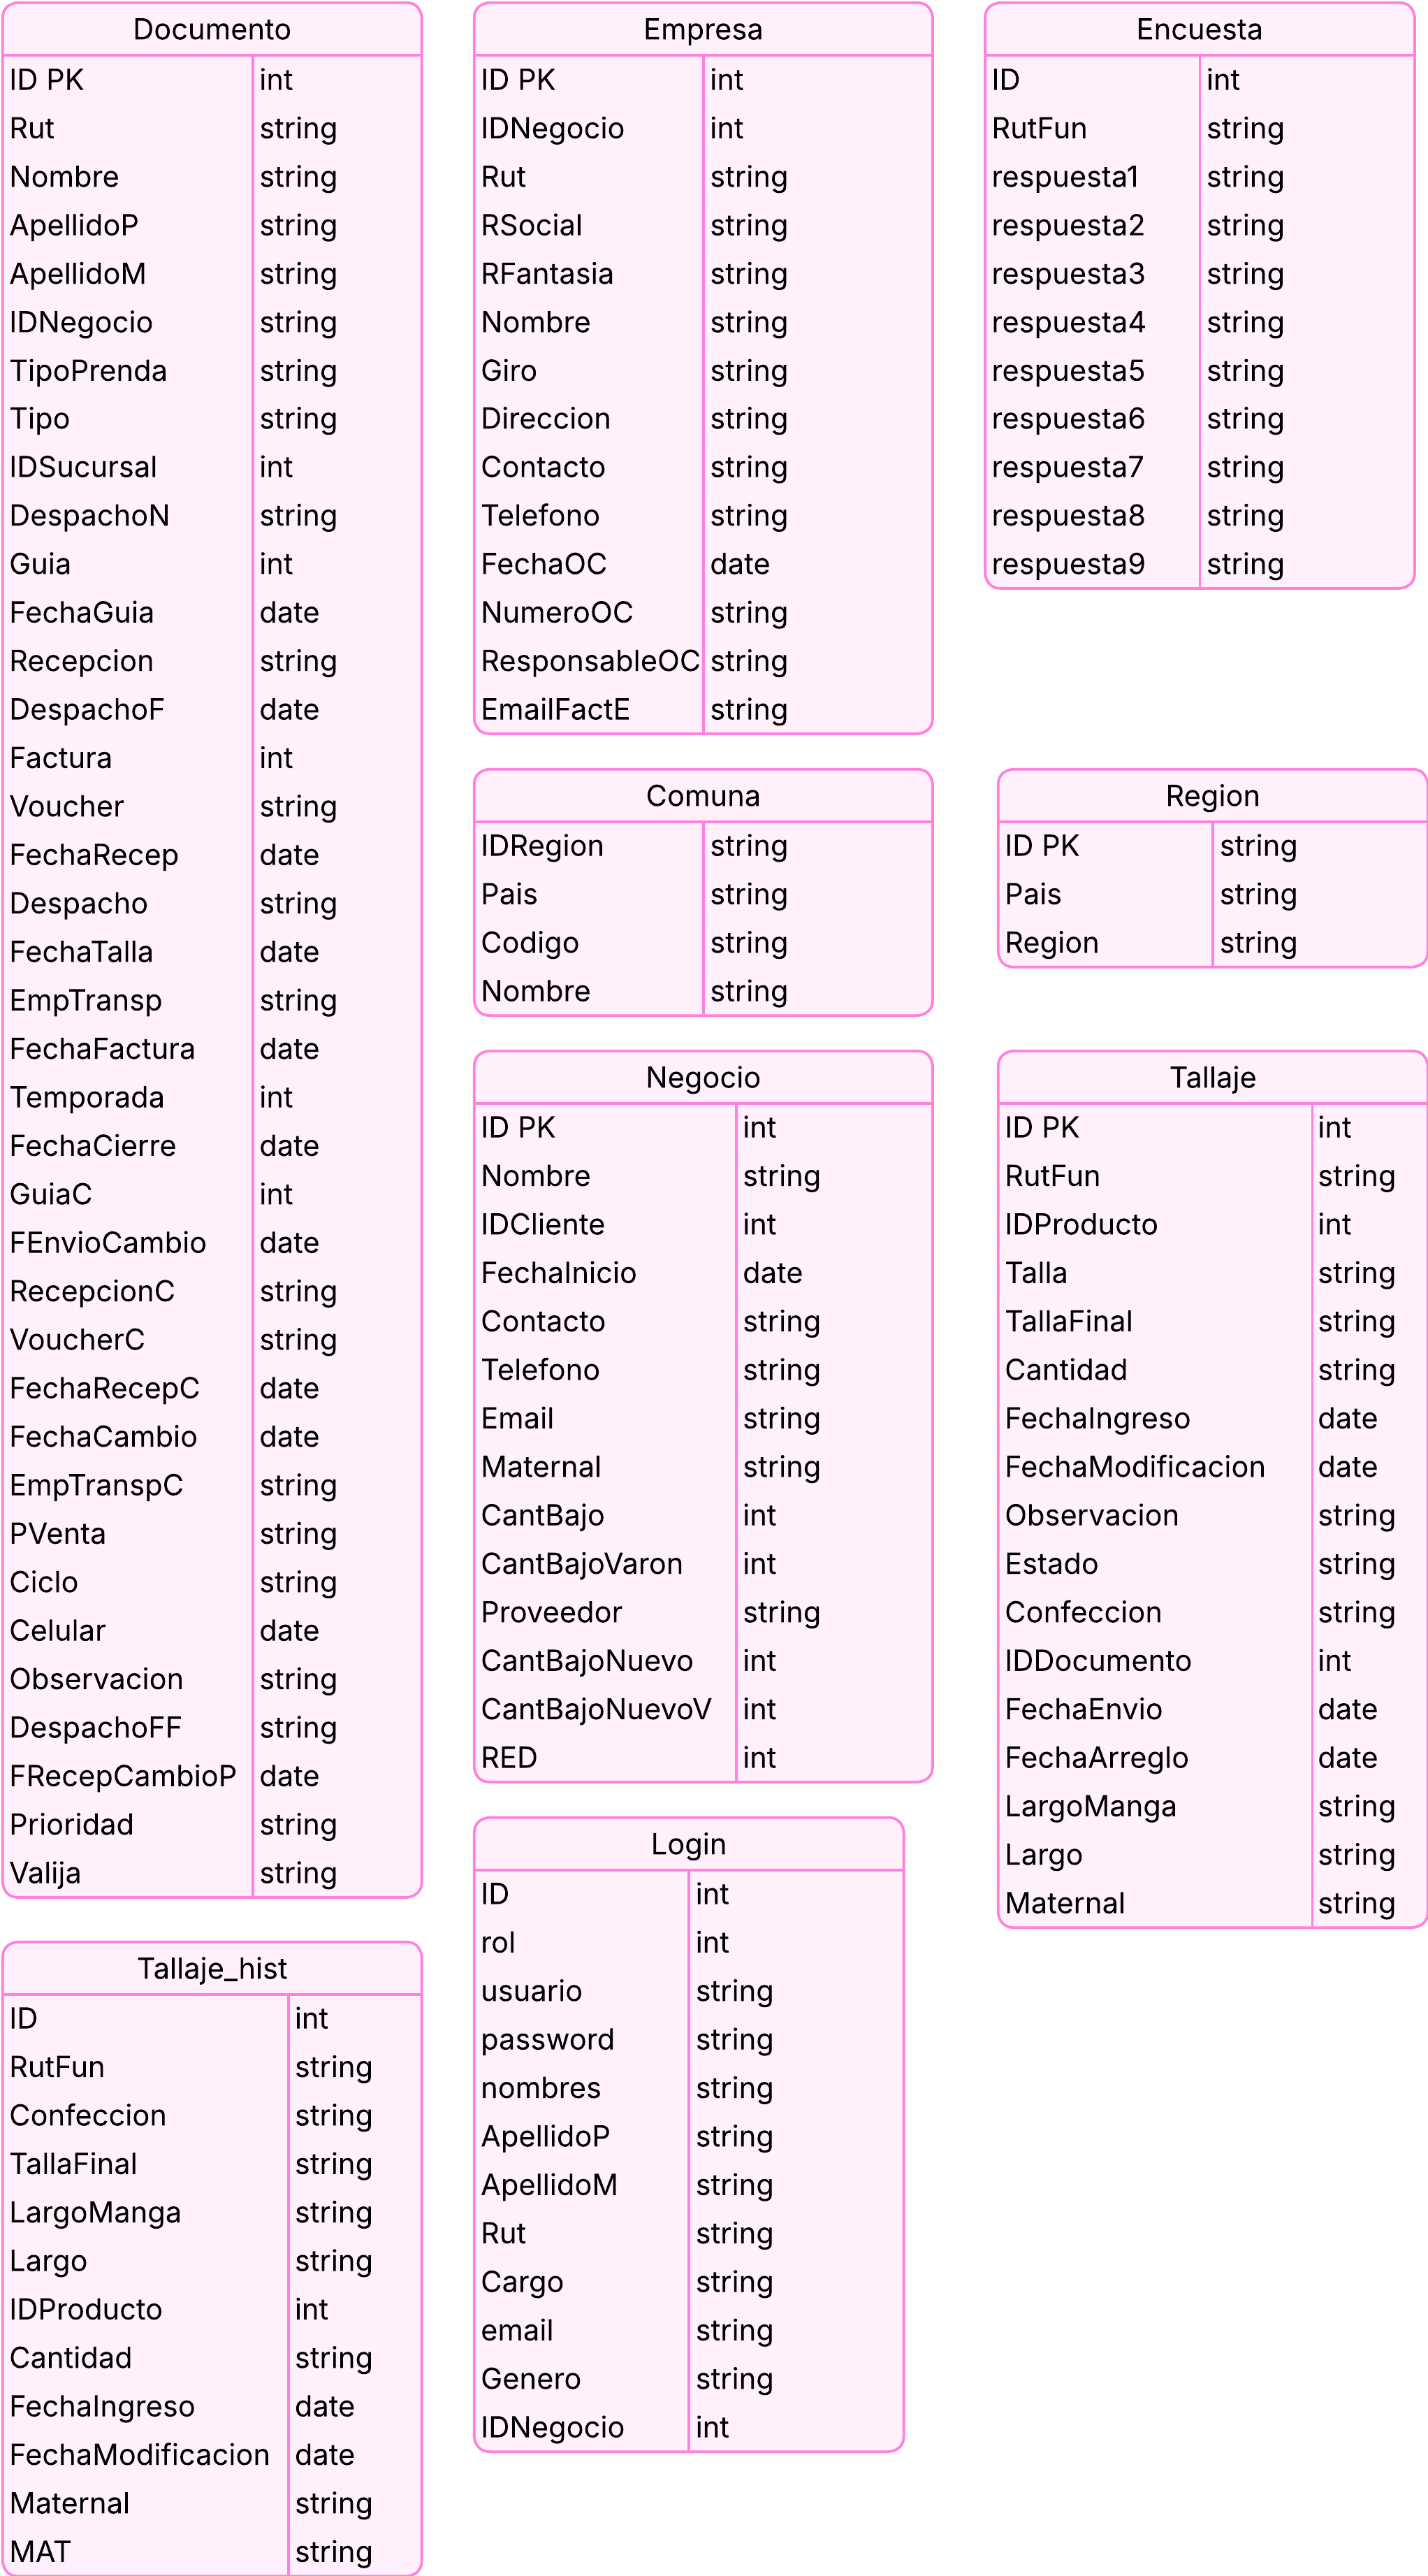
\includegraphics[height=0.7\textheight]{figuras/diagramas-actuales/diagrama-bdd-1}
    \caption{Diagrama físico de bases de datos del sistema actual (Parte 1)}
    \label{fig:diagrama-bdd-1-actual}
\end{figure}

\begin{figure}[htbp]
    \centering
    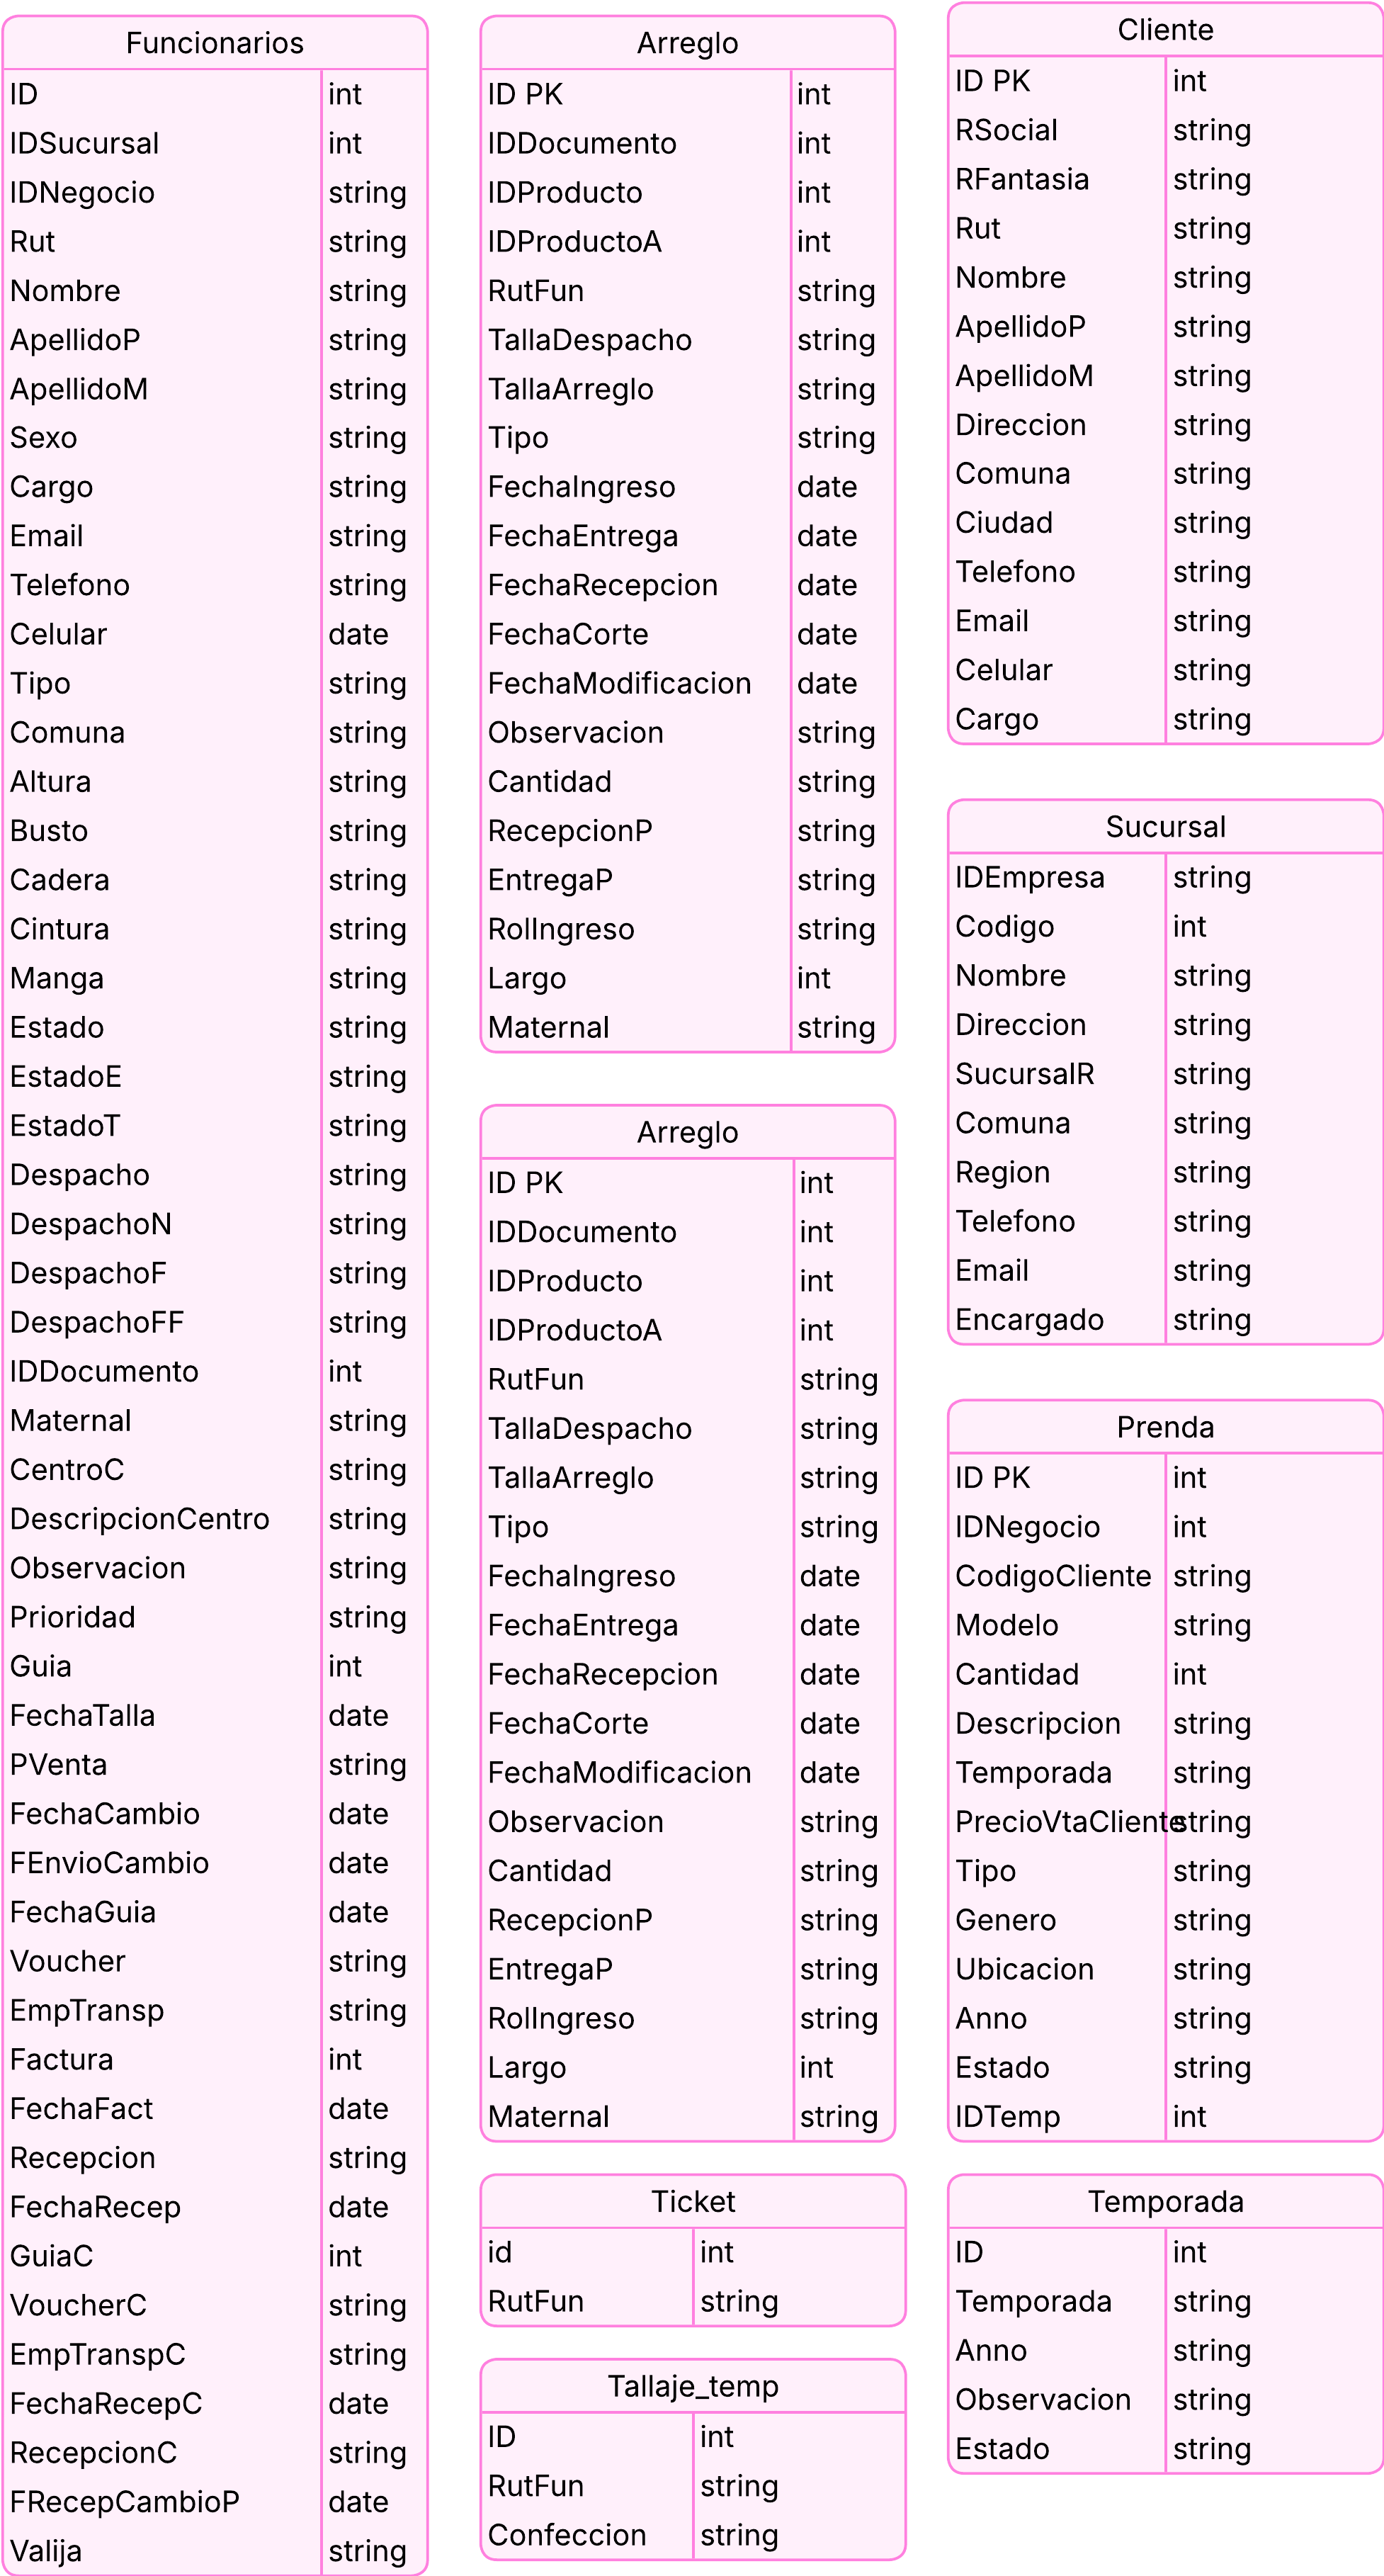
\includegraphics[height=0.7\textheight]{figuras/diagramas-actuales/diagrama-bdd-2}
    \caption{Diagrama físico de bases de datos del sistema actual (Parte 2)}
    \label{fig:diagrama-bdd-2-actual}
\end{figure}


\subsection{Diagrama de Flujo}

\subsection{Diagrama de Arquitectura}

\begin{figure}[htbp]
    \centering
    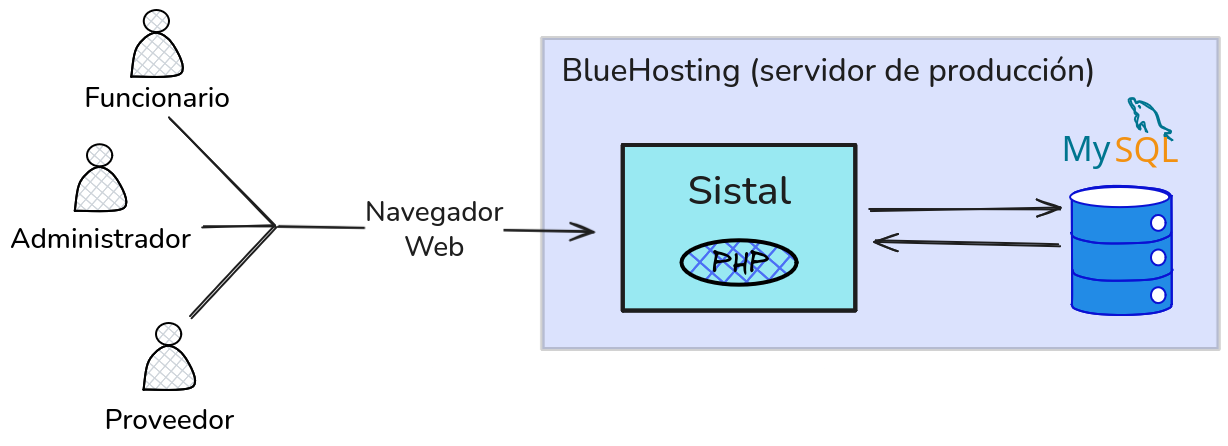
\includegraphics[width=0.9\textwidth]{figuras/diagramas-actuales/diagrama-de-arquitectura}
    \caption{Diagrama de arquitectura del sistema actual}
    \label{fig:diagrama-arq-actual}
\end{figure}

\subsection{Diagrama de Despliegue}

\begin{figure}[htbp]
    \centering
    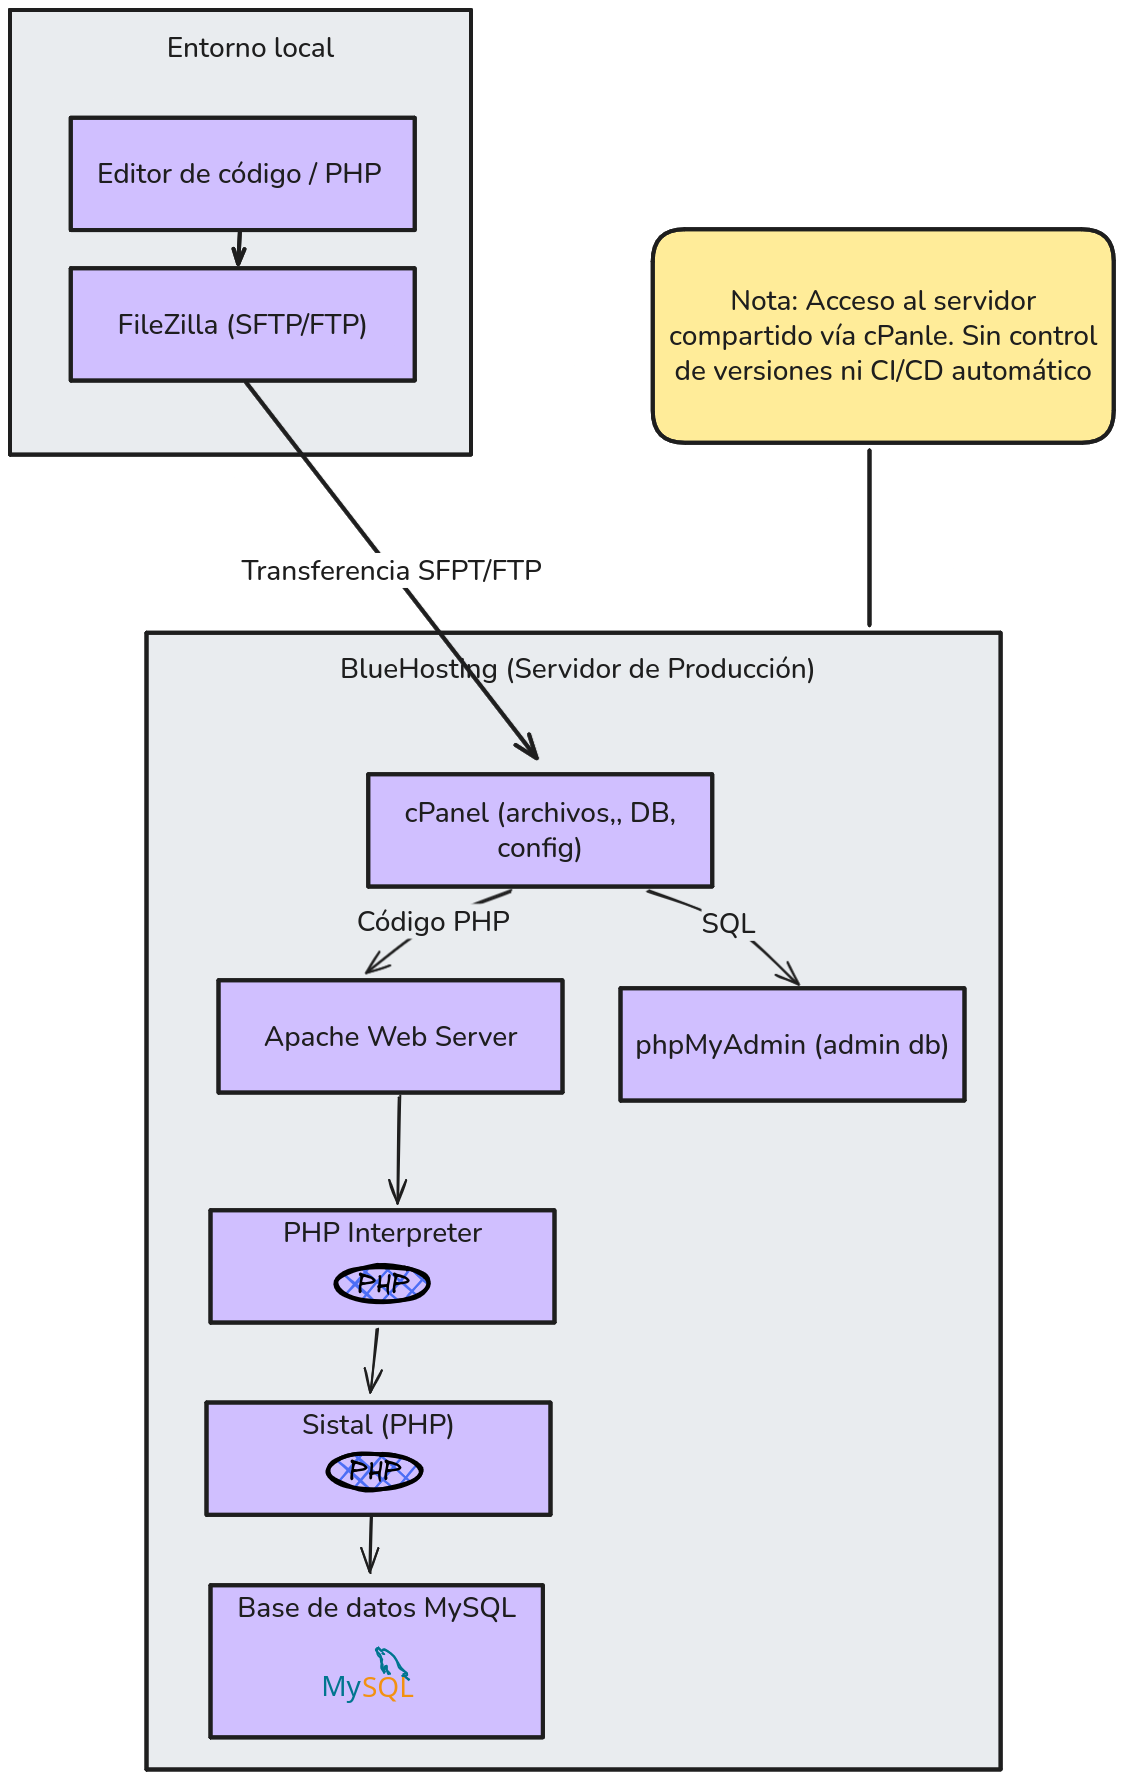
\includegraphics[width=0.5\textwidth]{figuras/diagramas-actuales/diagrama-de-despliegue}
    \caption{Diagrama de despliegue del sistema actual}
    \label{fig:diagrama-despliegue-actual}
\end{figure}



    \chapter*{Conclusiones}
\addcontentsline{toc}{chapter}{Conclusiones}

\textit{Pendiente...}

% Las conclusiones pueden incluir los resultados obtenidos en la investigación, comprobación o refutación de la hipótesis, recomendaciones que puedan ser útiles al problema de investigación, reflejando a su vez los alcances y limitaciones del trabajo, aportes al campo o disciplina del conocimiento y conclusiones generales.
% 
% Deben tener una redacción clara, concreta y directa; no son un resumen de la investigación.


    % \chapter{Cheatsheet}

% Formato de texto
\textbf{Negrita}, \textit{Itálica}, \underline{Subrayado}  

% Listas
\begin{itemize}
    \item Primer ítem
    \item Segundo ítem
\end{itemize}

\begin{enumerate}
    \item Ítem 1
    \item Ítem 2
\end{enumerate}

% Ecuaciones
Ecuación en la misma línea: $a^2 + b^2 = c^2$

Ecuación en medio: $$E = mc^2$$

% Figuras
\begin{figure}[htbp]
    \centering
    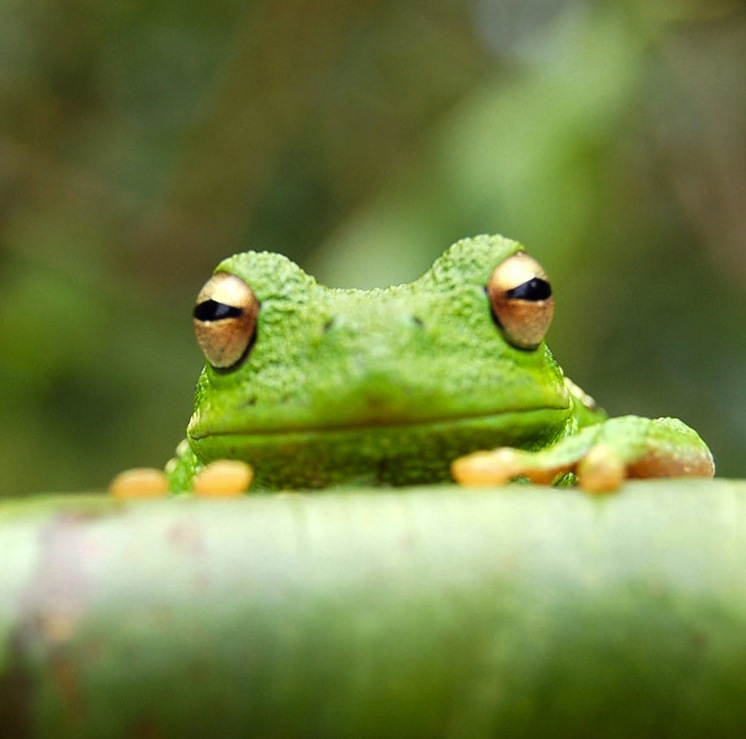
\includegraphics[width=0.3\linewidth]{figuras/frog.jpg}
    \caption{Ejemplo de cómo presentar una ilustración utilizando una foto del monumento a la brigada del Negev}
    \label{fig:ejemplo}
    \sourcefig{Israel Tour Guides}{2013}{https://israel-tourguide.info/2013/04/20/photo-of-the-week-negev-brigade-monument}
\end{figure}

% Tablas
\begin{table}[htbp]
    \centering
    \caption{Tabla de ejemplo}
    \begin{tabular}{|c|c|c|}
    \hline
    A & B & C \\ \hline
    1 & 2 & 3 \\ \hline
    4 & 5 & 6 \\ \hline
    \end{tabular}
    \label{tab:ejemplo}
\end{table}

% Referencias cruzadas
Ver Figura \ref{fig:ejemplo} y Tabla \ref{tab:ejemplo}.

% Citas y bibliografía
Ejemplo de cita: \cite{dinosaurios2006}; \parencite{dinosaurios2006}

% Enlaces
Ejemplo de enlace: \href{https://www.overleaf.com}{Overleaf}

Ejemplo de url: \url{https://www.overleaf.com}

% Código
\begin{lstlisting}[language=Python, caption=Hola Mundo en Python]
def saludo():
    print("Hola, mundo!")

saludo()
\end{lstlisting}

\begin{sloppypar}
    Palabras monoespaciadas: El directorio \code{\%HOME} se encuentra en \code{/home/<usuario>}
\end{sloppypar}

    % ================ Bibliografía ====================

    \printbibliography[heading=bibintoc]

    % ================ Glosario ========================

    % ================ Apendice ========================
    % Apendice
    % \include{apendice}

\end{document}
